%
%===============>> ГРУППА 9-1 МОДУЛЬ 3 <<=============
%
\setmodule{3}
%
%===============>>  Занятие 1  <<===============
%
\begin{class}[number=1]
	\begin{listofex}
		\item Для объектов, указанных в таблице, определите, какими цифрами они обозначены на плане. Заполните таблицу, в ответ запишите последовательность четырех цифр.
		\begin{center}
			\footnotesize
			\begin{tabular}{|g|c|c|c|c|}
				\hline
				\textbf{Объекты}&Книжный шкаф&Диван&Торшер&Стул\\
				\hline
				\textbf{Цифры}&&&&\\
				\hline
			\end{tabular}
		\end{center}
		\begin{center}
			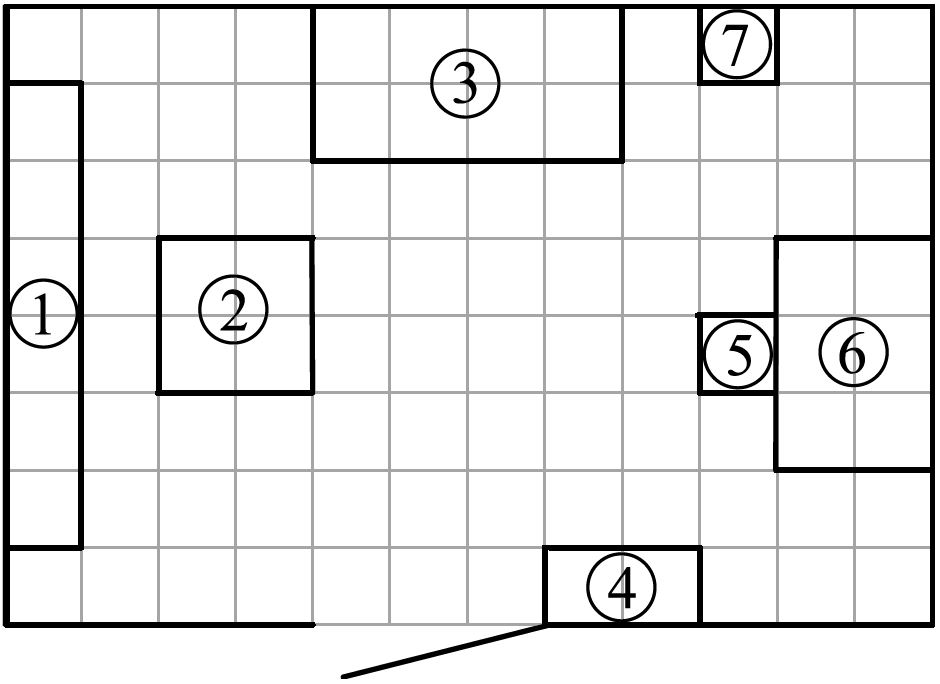
\includegraphics[align=t, width=0.3\textwidth]{pics/G91M3C2-1}
		\end{center}
	
		Владелец собирается провести ремонт своей квартиры. На плане изображена предполагаемая расстановка
		мебели в гостиной после ремонта. Сторона каждой клетки равна \( 0,4 \) м. Гостиная имеет прямоугольную
		форму. Единственная дверь гостиной деревянная, в стене напротив двери расположено окно. Справа от двери
		будет поставлен комод, слева от двери у стены будет собран книжный шкаф. В глубине комнаты у стены
		планируется поставить диван. Перед книжным шкафом будет поставлено кресло. Справа от дивана будет
		стоять торшер. Площадь, занятая диваном, по плану будет равна \( 1,28 \) м\( ^2 \). У стены справа от двери
		планируется поставить письменный стол, а перед ним поставить стул. Пол гостиной (в том числе там, где
		будет стоять мебель) планируется покрыть паркетной доской размером \( 40 \) см \( \times \) \( 20 \) см. Кроме того, владелец
		квартиры планирует смонтировать в гостиной электрический подогрев пола. Чтобы сэкономить, владелец не
		станет подводить обогрев под книжный шкаф, кресло, диван и комод, а также на участок площадью \( 0,16 \) м\( ^2 \)
		между диваном и торшером.
		\item Паркетная доска продаётся в упаковках по \( 15 \) штук. Сколько упаковок с паркетной доской нужно
		купить, чтобы покрыть пол гостиной?
		\item Найдите площадь той части гостиной, на которой будет смонтирован электрический подогрев пола. Ответ дайте в м\( ^2 \).
		\item Найдите расстояние d между противоположными углами кресла (диагональ). Ответ дайте в метрах в формате \( \dfrac{d}{\sqrt{2}} \).
		\item Владелец квартиры выбирает торшер из двух моделей \( A \) и \( B \). Цена торшеров и их среднее суточное потребление электроэнергии указаны в таблице. Цена электроэнергии составляет \( 4 \) рубля за кВт \( \cdot \) ч.
		\begin{center}
			\footnotesize
			\begin{tabular}{|c|c|x{8cm}|}
				\hline
				\rowcolor{gray}\textbf{Модель}&\textbf{Цена торшера (руб.)}&\textbf{Среднее потребление электроэнергии в сутки, кВт \( \cdot \) ч}\\
				\hline
				\( A \)&\( 2\:000 \)&\( 0,2 \)\\
				\hline
				\( B \)&\( 1\:200 \)&\( 0,3 \)\\
				\hline
			\end{tabular}
		\end{center}
		Обдумав оба варианта, владелец квартиры выбрал модель \( A \). Через сколько лет непрерывной работы экономия от меньшего расхода электроэнергии окупит разницу в цене этих торшеров? Ответ округлите до целого числа в большую сторону.
		\item Пользуясь описанием, определите, какими цифрами на плане обозначены населённые пункты. В ответ запишите последовательность трёх цифр без пробелов, запятых и других дополнительных символов.
		\begin{center}
			\footnotesize
			\begin{tabular}{|g|c|c|c|}
				\hline
				\textbf{Населенные пункты}&д. Камышевка&д. Ясная&д. Хомяково\\
				\hline
				\textbf{Цифры}&&&\\
				\hline
			\end{tabular}
		\end{center}
	
		Полина летом отдыхает у дедушки в деревне Ясная. В четверг они собираются съездить на велосипедах в
		село Майское в магазин. Из деревни Ясная в село Майское можно проехать по прямой лесной дорожке. Есть
		более длинный путь: по прямолинейному шоссе через деревню Камышёвка до деревни Хомяково, где нужно
		повернуть под прямым углом налево
		на другое шоссе, ведущее в село Майское. Есть и третий маршрут: в деревне Камышёвка можно свернуть на
		прямую тропинку в село Майское, которая идёт мимо пруда.
		Лесная дорожка и тропинка образуют с шоссе прямоугольные треугольники.
		\begin{center}
			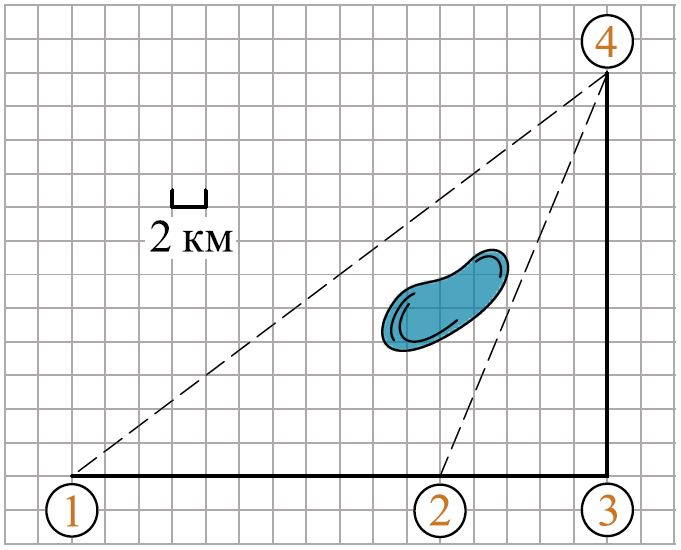
\includegraphics[align=t, width=0.3\textwidth]{pics/G91M3C2-2}
		\end{center}
		По шоссе Полина с дедушкой едут со скоростью 20 км/ч, а по лесной дорожке и тропинке --- со
		скоростью \( 15 \) км/ч. На плане изображено взаимное расположение населенных пунктов, длина стороны каждой клетки равна \( 2 \) км.
		\item Сколько километров проедут Полина с дедушкой от деревни Ясная до села Майское, если они поедут по шоссе через деревню Хомяково?
		\item Найдите расстояние от деревни Ясная до села Майское по прямой. Ответ дайте в километрах.
		\item Сколько минут затратят на дорогу из деревни Ясная в село Майское Полина с дедушкой, если поедут через деревню Хомяково?
		\item В таблице указана стоимость (в рублях) некоторых продуктов в четырех магазинах, расположенных в деревне Ясная, селе Майское, деревне Камышёвка и деревне Хомяково.
		\begin{center}
			\footnotesize
			\begin{tabular}{|c|c|c|c|c|}
				\hline
				\rowcolor{gray}\textbf{Продукт}&\textbf{д. Ясная}&\textbf{с. Майское}&\textbf{д. Камышевка}&\textbf{д. Хомяково}\\
				\hline
				Молоко (1 л)&42&38&41&33\\
				\hline
				Хлеб (1 батон)&25&21&29&30\\
				\hline
				Сыр Российский (1 кг)&310&320&290&280\\
				\hline
				Говядина (1 кг)&340&380&410&390\\
				\hline
				Картофель (1 кг)&15&20&17&18\\
				\hline
			\end{tabular}
		\end{center}
		Полина с дедушкой хотят купить \( 2 \) л молока, \( 3 \) кг говядины и \( 2 \) кг картофеля. В каком магазине такой набор продуктов будет стоить дешевле всего? В ответ запишите стоимость данного набора в этом магазине.
		\item \exercise{211}
		\item \exercise{445}
		\item \exercise{647}
	\end{listofex}
\end{class}
%
%===============>>  Домашняя работа 1  <<===============
%
\begin{homework}[number=1]
	\begin{listofex}
		\item Для объектов, указанных в таблице, определите, какими цифрами они обозначены на плане. Заполните таблицу, в ответ запишите последовательность четырех цифр.
		\begin{center}
			\footnotesize
			\begin{tabular}{|g|c|c|c|c|}
				\hline
				\textbf{Объекты}&Балкон&Детская комната&Кабинет&Кухня\\
				\hline
				\textbf{Цифры}&&&&\\
				\hline
			\end{tabular}
		\end{center}
		\begin{center}
			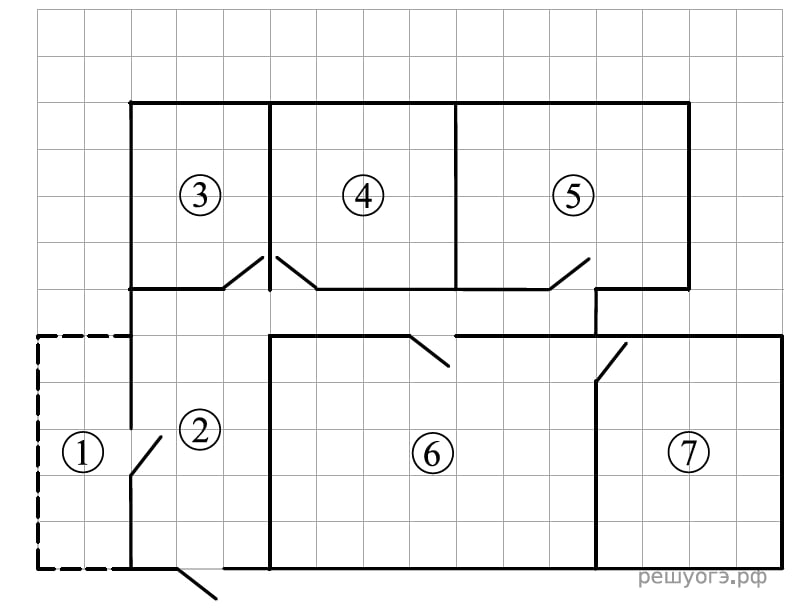
\includegraphics[align=t, width=0.3\textwidth]{pics/G91M3H1-1}
		\end{center}
			На плане изображена схема квартиры (сторона каждой клетки на схеме равна \( 1  \) м). Вход и выход
			осуществляются через единственную дверь.\\
			При входе в квартиру расположен коридор, отмеченный цифрой \( 2 \). Слева от него расположен балкон.
			Напротив входа в квартиру располагается совмещённый санузел, а справа от него — детская комната.
			Гостиная занимает наибольшую площадь в квартире, из гостиной можно попасть в кабинет. В конце
			коридора находится кухня площадью \( 20 \) м\( ^2 \).\\
			Пол в гостиной планируется покрыть паркетной доской длиной \( 1 \) м и шириной \( 0,25 \) м.
			В квартире проведены газопровод и электричество.
		\item Паркетная доска продаётся в упаковках по \( 8  \) шт. Сколько упаковок с паркетной доской требуется купить,
		чтобы покрыть пол в гостиной?
		\item Найдите площадь коридора (коридором считается площадь квартиры, не занятая комнатами или
		балконом). Ответ дайте в квадратных метрах.
		\item Найдите расстояние \( d  \) между противоположными углами детской комнаты в метрах. В ответ запишите \( \dfrac{d}{\sqrt{2}} \).
		\item Хозяин квартиры планирует установить в квартире счётчик. Он рассматривает два варианта:
		однотарифный или двухтарифный счётчики. Цены на оборудование и стоимость его установки, данные о
		потребляемой мощности, и тарифах оплаты даны в таблице.
	%		\begin{center}
	%		\footnotesize
	%		\begin{tabular}{|c|c|c|c|}
	%			\hline
	%			\rowcolor{gray}\textbf{}&\textbf{Оборудование и монтаж}&\textbf{Cред.потребл.мощность (в час)}&\textbf{Стоимость оплаты}\\
	%			\hline
	%			Однотарифный&\( 4 000 \) руб.&\( 6 \)кВт&\( 5 \) руб./(кВт\( \cdot \)ч)\\
	%			\hline
	%			Двухтарифный&\( 8 200 \) руб.&\multirow{\( 6 \)кВт}&\( 5 \) руб./(кВт\( \cdot \)ч) днём \\
	%			\cline{4-4}
	%			&&& \( 3 \) руб./(кВт\( \cdot \)ч) ночью \\
	%			\hline
	%		\end{tabular}
	%	\end{center}
	\begin{center}
		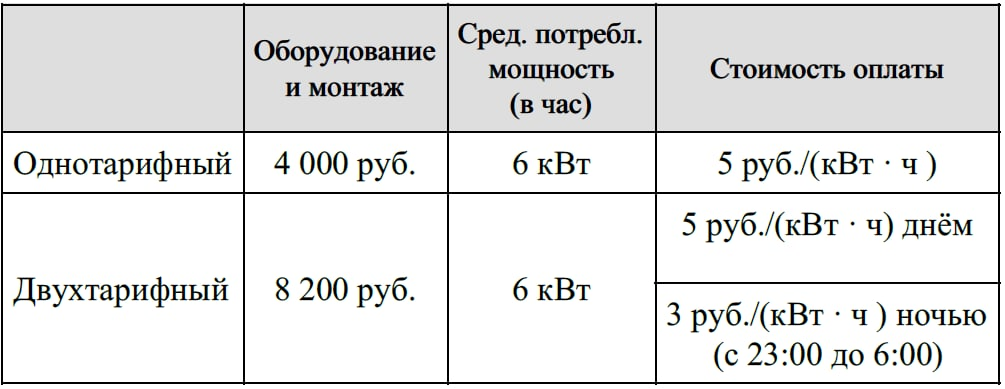
\includegraphics[align=t, width=0.7\textwidth]{pics/G91M3H1-2}
	\end{center}
	Обдумав оба варианта, хозяин решил установить двухтарифный электросчётчик. Через сколько дней
	непрерывного использования электричества экономия от использования двухтарифного счётчика вместо
	однотарифного компенсирует разность в стоимости установки двухтарифного счётчика и однотарифного?
	\item На экзамене \( 50 \) билетов, Руслан не выучил \( 5 \) из них. Найдите вероятность того, что ему попадется
	выученный билет.
	\item Игральную кость бросают один раз. Найдите вероятность того, что выпало число, большее \( 3 \).
	\item Стас, Денис, Костя, Маша, Дима бросили жребий -- кому начинать игру. Найдите вероятность того, что
	начинать игру должна будет девочка.
	\item Определите вероятность того, что при бросании игрального кубика (правильной кости) выпадет нечетное
	число очков.
	\item \exercise{1478}
	\end{listofex}
\end{homework}
%
%
%===============>>  Занятие 4  <<===============
%
\begin{class}[number=4]
	\begin{listofex}
		\item В таблице даны размеры (с точностью до мм) четырёх листов, имеющих форматы А0, А1, А3 и А4.
		\begin{center}
			\footnotesize
			\begin{tabular}{|c|c|c|}
				\hline
				\rowcolor{gray}\textbf{Номер листа}&\textbf{Длина (мм)}&\textbf{Ширина (мм)}\\
				\hline
				\( 1 \)&\( 297 \)&\( 210 \)\\
				\hline
				\( 2 \)&\( 420 \)&\( 297 \)\\
				\hline
				\( 3 \)&\( 1189 \)&\( 841 \)\\
				\hline
				\( 4 \)&\( 841 \)&\( 594 \)\\
				\hline
			\end{tabular}
		\end{center}
		Установите соответствие между форматами и номерами листов. В ответ запишите последовательность четырёх цифр, соответствующих номерам листов, без пробелов, запятых и дополнительных символов.
			\begin{center}
			\footnotesize
			\begin{tabular}{|c|c|c|c|}
				\hline
				\rowcolor{gray}А0&А1&А3&А4\\
				\hline
				&&&\\
				\hline
			\end{tabular}
		\end{center}
		Общепринятые форматы листов бумаги обозначают буквой А и цифрой: А0, А1, А2 и так далее. Лист формата А0 имеет форму прямоугольника, площадь которого равна 1 кв. м. Если лист формата А0 разрезать пополам параллельно меньшей стороне, получается два равных листа формата А1. Если лист А1 разрезать так же пополам, получается два листа формата А2. И так далее.
		\begin{center}
			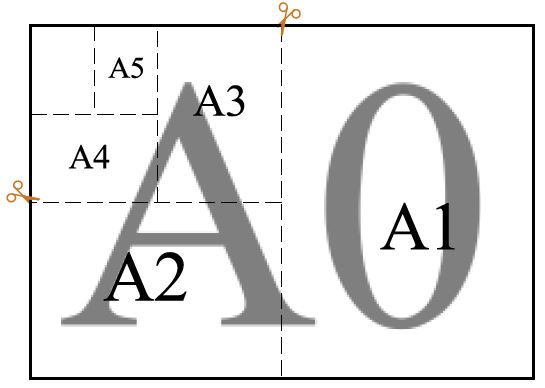
\includegraphics[align=t, width=0.3\textwidth]{pics/G91M3C4-1}
		\end{center}
		Отношение большей стороны к меньшей стороне листа каждого формата одно и то же, поэтому листы всех форматов подобны. Это сделано специально для того, чтобы пропорции текста и его расположение на
		листе сохранялись при уменьшении или увеличении шрифта при изменении формата листа.
		\item Сколько листов формата А3 получится из одного листа формата А2?
		\item Найдите площадь листа формата А1. Ответ дайте в квадратных сантиметрах.
		\item Найдите отношение длины меньшей стороны листа формата А3 к большей. Ответ округлите до
		десятых.
		\item Бумагу формата А5 упаковали в пачки по 500 листов. Найдите массу пачки, если масса бумаги
		площади 1 кв. м равна 80 г. Ответ дайте в граммах.
		\item Миша выбирает трехзначное число. Найдите вероятность того, что оно делится на 2.\answer{\( 0,5 \)}
		\item Определите вероятность того, что при бросании кубика выпало число очков, не меньше 4.\answer{\( 0,5 \)}
		\item В среднем из каждых 80 поступивших в продажу аккумуляторов 76 аккумуляторов заряжены. Найдите вероятность того, что купленный аккумулятор не заряжен.\answer{\( 0,05 \)}
		\item Из каждых 1000 электрических лампочек 5 бракованных. Какова вероятность купить исправную лампочку?\answer{\( 0,995 \)}
		\item Для экзамена подготовили билеты с номерами от 1 до 50. Какова вероятность того, что наугад взятый учеником билет имеет однозначный номер?\answer{\( 0,18 \)}
		\item В мешке содержатся жетоны с номерами от 5 до 54 включительно. Какова вероятность, того, что извлеченный наугад из мешка жетон содержит двузначное число?\answer{\( 0,9 \)}
		\item В таблице представлены результаты четырёх стрелков, показанные ими на тренировке.
		\begin{center}
			\footnotesize
			\begin{tabular}{|c|c|c|}
				\hline
				\rowcolor{gray}\textbf{Номер стрелка}&\textbf{Число выстрелов}&\textbf{Число попаданий}\\
				\hline
				\( 1 \)&\( 42 \)&\( 28 \)\\
				\hline
				\( 2 \)&\( 70 \)&\( 20 \)\\
				\hline
				\( 3 \)&\( 54 \)&\( 45 \)\\
				\hline
				\( 4 \)&\( 46 \)&\( 42 \)\\
				\hline
			\end{tabular}
		\end{center}
		
		Тренер решил послать на соревнования того стрелка, у которого относительная частота попаданий выше. Кого из стрелков выберет тренер? Укажите в ответе его номер.\answer{\( 4 \)}
		\item В магазине канцтоваров продаётся 100 ручек, из них 37 --- красные, 8 --- зелёные, 17 --- фиолетовые, ещё есть синие и чёрные, их поровну. Найдите вероятность того, что Алиса наугад вытащит красную или чёрную ручку.\answer{\( 0,56 \)}
		\item Вычислить:
		\begin{enumcols}[itemcolumns=3]
			\item \exercise{1724}
			\item \exercise{1774}
			\item \exercise{1747}
		\end{enumcols}
		\item \exercise{1035}
	\end{listofex}
\end{class}
%
%===============>>  Домашняя работа 2  <<===============
%
\begin{homework}[number=2]
	\begin{listofex}
		\item Игорь страховал свою гражданскую ответственность три года. В течение первого года была сделана одна
		страховая выплата, после этого выплат не было. Какой класс будет присвоен Игорю на начало четвёртого
		года страхования?\\
		Каждый водитель в Российской Федерации должен быть застрахован по программе обязательного
		страхования гражданской ответственности (ОСАГО). Стоимость полиса получается умножением базового
		тарифа на несколько коэффициентов. Коэффициенты зависят от водительского стажа, мощности автомобиля,
		количества предыдущих страховых выплат и других факторов.\\
		Коэффициент бонус-малус (КБМ) зависит от класса водителя. Это коэффициент, понижающий или
		повышающий стоимость полиса в зависимости от количества ДТП в предыдущий год. Сначала водителю
		присваивается класс 3. Срок действия полиса, как правило, один год. Каждый последующий год класс
		водителя рассчитывается в зависимости от числа страховых выплат в течение истекшего года, в соответствии
		со следующей таблицей.\\
		\begin{center}
			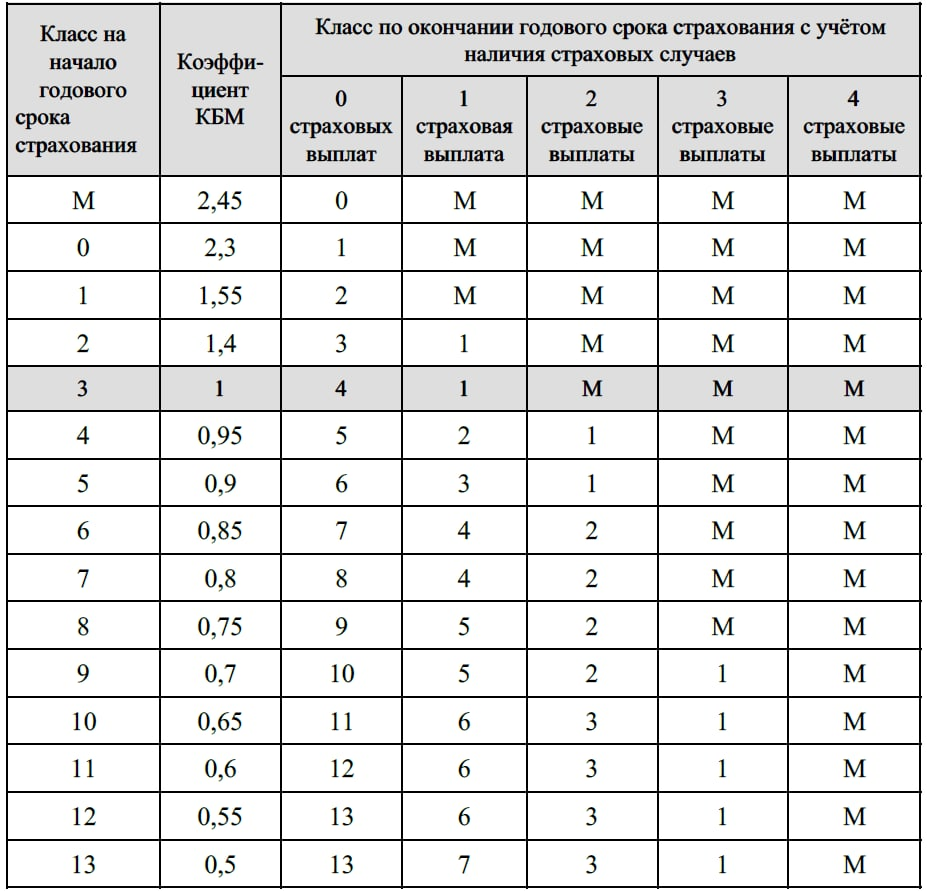
\includegraphics[align=t, width=0.8\textwidth]{pics/G91M3H2-1}
		\end{center}
%			\begin{center}
%			\footnotesize
%			\begin{tabular}{|l|l|l|}
%				\hline
%				\multicolumn{2}{|c|}{Multi-Column} & Column 3 \\
%				\hline
%				Column 1 & Column 2 & Column 3 \\
%				\hline
%			\end{tabular}
%		\end{center}
	\item Чему равен КБМ на начало четвёртого года страхования?
	\item Коэффициент возраста и водительского стажа (КВС) также влияет на стоимость полиса (см. таблицу).
	\begin{center}
		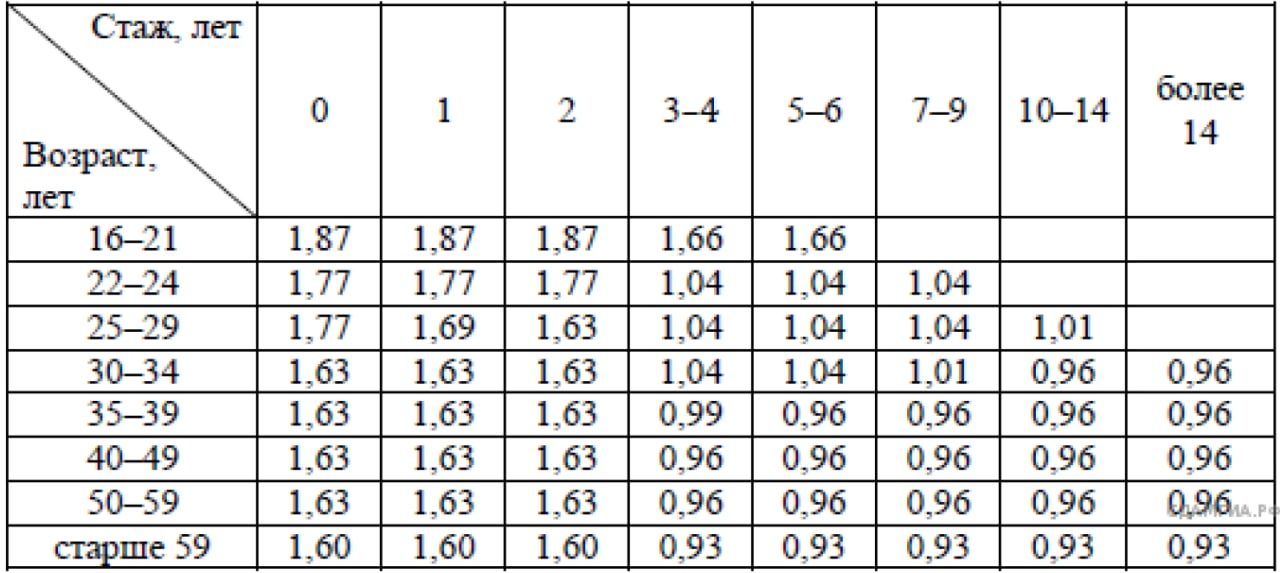
\includegraphics[align=t, width=0.8\textwidth]{pics/G91M3H2-2}
	\end{center}
		Когда Игорь получил водительские права и впервые оформил полис, ему было \( 22 \) года. Чему равен КВС на начало \( 4 \)-го года страхования?
	\item В начале третьего года страхования Игорь заплатил за полис \( 18 585 \) руб. Во сколько рублей обойдётся Игорю полис на четвёртый год, если значения других коэффициентов (кроме КБМ и КВС) не изменятся?	
	\item Игорь въехал на участок дороги протяжённостью \( 2,6 \) км с камерами, отслеживающими среднюю скорость движения. Ограничение скорости на дороге -- \( 100  \) км/ч. В начале и в конце участка установлены камеры, фиксирующие номер автомобиля и время проезда. По этим данным компьютер вычисляет среднюю скорость на участке. Игорь въехал на участок в \( 11:10:33 \), а покинул его в \( 11:11:51 \). Нарушил ли Игорь скоростной режим? Если да, на сколько км/ч средняя скорость на данном участке была выше разрешённой?
	\item Решите уравнение \( \dfrac{5x+4}{2}+3=\dfrac{9x}{4} \)
	\item Решите уравнение \( 2x^2-10x=0 \)
	\item \exercise{1510}
	\item Стас, Денис, Костя, Маша, Дима бросили жребий -- кому начинать игру. Найдите вероятность того, что начинать игру должна будет девочка.
	\item Известно, что \( a<b<0 \). Выберите наименьшее из чисел.
	\begin{enumcols}[itemcolumns=1]
		\item \( a-1 \)
		\item \( b-1 \)
		\item \( ab \)
		\item \( -b \)
	\end{enumcols}
	\end{listofex}
\end{homework}
%
%===============>>  Занятие 5  <<===============
%
%\begin{class}[number=5]
%	\begin{listofex}
%	
%	\end{listofex}
%\end{class}
%
%===============>>  Занятие 6  <<===============
%
%\begin{class}[number=6]
%	\begin{listofex}
%	
%	\end{listofex}
%\end{class}
%
%===============>>  Домашняя работа 3  <<===============
%
%\begin{homework}[number=3]
%	\begin{listofex}
%
%	\end{listofex}
%\end{homework}
%\newpage
%\title{Подготовка к проверочной работе}
%\begin{listofex}
%	
%\end{listofex}
%
===============>>  Занятие 7  <<===============

\begin{class}[number=7]
	\begin{listofex}
	 \item пусто
	\end{listofex}
\end{class}
%
%===============>>  Провечная работа  <<===============
%
%\begin{exam}
%	\begin{listofex}
%	
%	\end{listofex}
%\end{exam}
%
%===============>>  Консультация  <<===============
%
\begin{consultation}
	\begin{listofex}
		\item Построить график функции:
		\begin{enumcols}[itemcolumns=2]
			\item \( y=x^2 \)
			\item \( y=(x+2)^2 \)
			\item \( y=(x-3)^2-2 \)
			\item \( y=x^2-4x+6 \)
			\item \( y=\sqrt{x} \)
			\item \( y=\sqrt{x}-1 \)
			\item \( y=\sqrt{x+3}-1 \)
		\end{enumcols}
		\item Принадлежит ли точка с координатами \( (16;6) \) графику функции \( y=\sqrt{x}+2 \)?
		\item Принадлежит ли точка с координатами \( (2;7) \) графику функции \( y=x^2-3x+7 \)?
		\item Найдите координаты точек пересечения прямой \( y=2x-7 \) и параболы \( y=x^2+8x+1 \).
		\item Построить график функции:\quad\( y=\dfrac{(x+3)^2(x-1)}{x+3}-2 \).
	\end{listofex}
\end{consultation}
%
%===============>>  Консультация  <<===============
%
\begin{consultation}
	\begin{listofex}
		\item Найдите значение выражения \( \dfrac{6^{\sqrt{3}}\cdot7^{\sqrt{3}}}{42^{\sqrt{3}-1}} \).
		\item Найдите значение выражения \( \dfrac{16x-25y}{4\sqrt{x}-5\sqrt{y}}-\sqrt{y} \), если \( \sqrt{x}+\sqrt{y}=3 \).
		\item Найдите значение выражения \( \dfrac{2\sin^2x-\sin x\cos x}{3\sin^2x+2\cos^2x} \), если \( \tg x = 2 \).
		\item Найдите значение выражения \( \log_a\dfrac{a^6}{b^4} \), если \( \log_a b = -2 \).
		\item В Волшебной стране бывает два типа погоды: хорошая и отличная, причём погода, установившись утром, держится неизменной весь день. Известно, что с вероятностью 0,8 погода завтра будет такой же, как и сегодня. Сегодня 3 июля, погода в Волшебной стране хорошая. Найдите вероятность того, что 6 июля в Волшебной стране будет отличная погода.
		\item Чтобы поступить в институт на специальность «Лингвистика», абитуриент должен набрать на ЕГЭ не менее \( 70 \) баллов по каждому из трёх предметов --- математика, русский язык и иностранный язык. Чтобы поступить на специальность «Коммерция», нужно набрать не менее \( 70 \) баллов по каждому из трёх предметов --- математика, русский язык и обществознание.
		
		Вероятность того, что Мария получит не менее \( 70 \) баллов по математике, равна \( 0,6 \), по русскому языку --- \( 0,8 \), по иностранному языку --- \( 0,7 \) и по обществознанию --- \( 0,5 \).
		
		Найдите вероятность того, что Мария сможет поступить хотя бы на одну из двух упомянутых специальностей.
		\item Два велосипедиста одновременно отправились в 240-километровый пробег. Первый ехал со скоростью, на 1 км/ч большей, чем скорость второго, и прибыл к финишу на 1 час раньше второго. Найти скорость велосипедиста, пришедшего к финишу первым. Ответ дайте в км/ч.
		\item Смешали некоторое количество 15\%-го раствора некоторого вещества с таким же количеством 19\%-го раствора этого вещества. Сколько процентов составляет концентрация получившегося раствора?
		\item Изюм получается в процессе сушки винограда. Сколько килограммов винограда потребуется для получения 20 килограммов изюма, если виноград содержит 90\% воды, а изюм содержит 5\% воды?
	\end{listofex}
\end{consultation}
%
%===============>>  Консультация  <<===============
%
\begin{consultation}
	\begin{listofex}
		\item Найти сумму векторов:
		\begin{enumcols}[itemcolumns=2]
			\item \( \overline{a}=(-2;1) \) и \( \overline{a}=(5;3) \);
			\item \( \overline{m}=(-5;7) \) и \( \overline{n}=(6;-5) \);
			\item \( \overline{a}=(3;2) \); \( \overline{b}=(-1;4) \) и \( \overline{c}=(0;3) \).
		\end{enumcols}
		\item Найти координаты вектора \( 3\overline{a} \), если \( \overline{a}=(-4;1) \).
		\item Найти координаты вектора \( 2\overline{a}-0,5\overline{b} \), если \( \overline{a}=(2;7) \) и \( \overline{b}=(-12;6) \).
		\item Найти координаты вектора \( \overrightarrow{AB} \), если \( A(3;-1) \) \( B(1;-5) \).
		\item Найти длину вектора \( \overline{a}=(-4;3) \).
		\item Найти длину вектора \( \overrightarrow{AB} \), если \( A(2;4) \) \( B(8;10) \).
		\item Известно, что \( A(0;2);\;B(-2;4);\;C(3;1);\;D(3;4);\;E(2;-1);\;F(6;2) \).
		\begin{enumcols}
			\item Изобразить вектора \( \overrightarrow{AC};\;\overrightarrow{BD};\; \overrightarrow{EA};\;\overrightarrow{CF};\;\overrightarrow{FB} \);
			\item Построить вектор, равный: \( \overrightarrow{AC}+\overrightarrow{BD};\;\overrightarrow{FD}+3\overrightarrow{EC};\;\overrightarrow{AF}+\overrightarrow{EC}+\overrightarrow{DB} \);
			\item Построить вектор, равный \( \overrightarrow{FA}+\overrightarrow{EC} \) и найти его длину;
			\item Построить вектор, равный: \( \overrightarrow{BD}-\overrightarrow{AE};\;\overrightarrow{DF}-\overrightarrow{AC}; \);
			\item Построить вектор, равный: \( \overrightarrow{AB}+\overrightarrow{BC}+\overrightarrow{AE}-\overrightarrow{ED} \).
		\end{enumcols}
	\end{listofex}
\end{consultation}
%
%===============>>  Консультация  <<===============
%
\begin{consultation}
	\begin{listofex}
		\item Решить уравнение:
		\begin{enumcols}[itemcolumns=1]
			\item \exercise{36}
			\item \exercise{1010}
			\item \exercise{554}
			\item \exercise{1032}
			\item \exercise{1023}
		\end{enumcols}
		\item Решить уравнение:
		\begin{enumcols}[itemcolumns=1]
			\item \exercise{995}
			\item \exercise{1037}
			\item \exercise{1004}
		\end{enumcols}
		\item \exercise{1023}
		\item \exercise{973}
	\end{listofex}
\end{consultation}
%
%===============>>  Консультация  <<===============
%
\begin{consultation}
	\begin{listofex}
		\item Решить неравенство:
		\begin{enumcols}[itemcolumns=2]
			\item \( (x-7)(2x+4)\ge0 \)
			\item \( (0,25x-4)(3-x)(x+5)<0 \)
			\item \( x(x+3,5)\le0 \)
		\end{enumcols}
		\item Решить неравенство:
		\begin{enumcols}[itemcolumns=2]
			\item \( x^2-3x>0 \)
			\item \( 4x2-3x\le2x^2+x\)
			\item \( x^2-9\ge0 \)
			\item \( 16x^2>81 \)
			\item \( \mfrac{3}{1}{2}x-x^2<0 \)
			\item \( 5-0,2x^2>0 \)
		\end{enumcols}
		\item Решить неравенство:
		\begin{enumcols}[itemcolumns=2]
			\item \exercise{647}
			\item \( 7x^2+2x-5>0 \)
			\item \( 0,25x^2-4x+12>0 \)
			\item \( x^2-5x+4>0 \)
		\end{enumcols}
		\item Решить неравенство:
		\begin{enumcols}[itemcolumns=2]
			\item \( (x-4)^2>0\)
			\item \( x^2-4x+4<0 \)
			\item \( x^2-2x+1\ge0 \)
			\item \( x^2-8x+16\le0 \)
		\end{enumcols}
	\end{listofex}
\end{consultation}